\begin{parag}{Ex hat party 1950}
    \begin{itemize}
        \item $n$ men, all have the same hat
        \item they throw hats in a corner
        \item leaving, they randomly take a hat
    \end{itemize}
    \begin{subparag}{Solution}
        Let $R_i = \begin{cases}
            1, \text{ if person } i \text{ leaves with their own hat} \\
            0, \text{ otherwise}
        \end{cases}$\\
    There we search the Expected value here:
    \begin{align*} 
        \mathbb{E}\left[R_1 + R_2 + \cdots + R_n\right] &= \mathbb{E}\left[R_1\right] + \mathbb{E}\left[R_2\right] + \cdots + \mathbb{E}\left[R_n\right]\\
                                                        &= \frac{1}{n} + \frac{1}{n} + \cdots + \frac{1}{n}\\
                                                        &= 1
    \end{align*}

   Then we know that, on average, only one person get the right hat.
    \end{subparag}

\end{parag}
\lecture{3}{2025-02-25}{suite}{}
\begin{parag}{Entropy}
    \begin{equation} H_2(S) =\sum_i p(s)\log \frac{1}{2p(s)} \end{equation}
    \begin{equation} = \frac{1}{8}\log_2 \frac{8}{2} + \frac{1}{8} \log_2 8 \end{equation}
   
    
    \begin{equation} \approx \frac{1}{8} + \frac{1}{8} \cdot 3 \end{equation}
    
  \begin{subparag}{personal remark}
      We can see it as an average of "surprise".
      \\
      Where the average is the randomness. ($\approx 0.55$)
  \end{subparag}  
\end{parag}

\subsection{Entropy bounds}

\begin{parag}{Bound}
    \begin{align*}
        0 \leq H_b(S) \leq \log_b \mathcal{A}
    \end{align*}
    
\end{parag}

    \section{Source Coding Purpose}
    Source coding is often seen as a way to compress the source.
    \\
    More generally, the foal of source coding is to efficiently describe how much information there is to a \textit{file}
    
 \subsection{Setup}
 \begin{parag}{Setup}
     The \textbf{encoder} is specified by:
     : \
\begin{itemize}
    \item the input alphabet$ \mathcal{A}$ (the same as the source alphabet)
    \item the output alphabet $\mathcal{D} $(typically  $ \mathcal{D} = \{0, 1\}$);
    \item the codebook $\mathcal{C} $ Which consists of finite sequences over $ \mathcal{D}$;
    \item By the one to one encoding map $ \Gamma : \mathcal{A}^k \to \mathcal{C}$ where $k$ is a positive integer.
\end{itemize}
For now, $k = 1$.


 \end{parag}
 
 \begin{parag}{Example}
     For each code, the encoding map $ \Gamma$ is specified in the following table:
     \begin{center}
         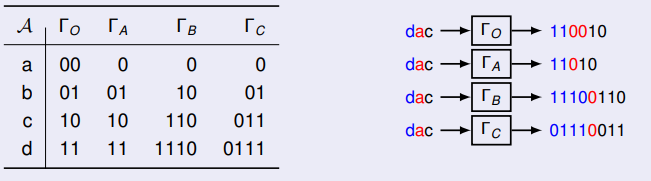
\includegraphics[scale=0.8]{12025-06-02.png}
     \end{center}
     
 
 \end{parag}
\begin{parag}{Decodability}
    We want to avoir the following problem (encoding map $\Gamma_A$ )
    \begin{align*}
        cbaad \to 100010011 \begin{cases} \to cbaad \\ \to cacad
    \end{align*}

    \begin{definition}
        The code is uniquely decodable if every concatenation of codewords has a unique parsing into a sequence of codewords.
    \end{definition}
    
    Recall that the encoding function $\Gamma$ is one to one by assumption
    \begin{subparag}{Example}
        Code $C$ or $B$ are uniquely decodable : 
        (A mettre une image 106)
    \end{subparag}
\end{parag}
 
\begin{parag}{Prefix Free codes}
    \begin{definition}
        If no codeword is a prefix of another codeword, the code is said to be prefix free.
    \end{definition}
   \begin{subparag}{Example}
        The codeword \important{01} is a prefix of \important{01}1. \\

       
   \end{subparag}
   \begin{itemize}
       \item A prefix free code is always uniquely decodable
       \item A uniquely decodable code is \important{not necessarily} prefix free
   \end{itemize}
   \begin{subparag}{A prefix code }
       A prefix free code is also called instantaneous code : 
       \begin{itemize}
           \item Think of phone numbers
           \item Think about streaming: instantaneous codes minimize the decoding delay (for given codeword length)
       \end{itemize}
   \end{subparag}
\end{parag}
 
\begin{parag}{Code for one random variable}
    We start by considering codes that encode \important{one single random variable} $ S \in \mathcal{A}$.
    \\
    To encode a sequence $S_1, S_2, \dots $ of random variables, we encode one random variable at a time.
\end{parag}

\begin{parag}{Complete tree of a code}
    Slide 113 screen.
\end{parag}
\begin{parag}{Binary tree}
    \begin{itemize}
        \item There is a \improtant{root} (the beginning)
        \item A vertex (another node)
        \item A \important{leaf} is the last vertex
        \item Which is like a (arbre généalogique)
    \end{itemize}
\end{parag}
\begin{parag}{Ternary Tree}
    The same as a binary tree but with three children.
\end{parag}

\begin{parag}{With/Without prefix}
slide 115.
\end{parag}

\begin{parag}{Decoding tree}
    \begin{itemize}
        \item Obtained from the complete tree by keeping only branches that form a codeword
        \item Useful to visualize the decoding process
    \end{itemize}
    Slide 116
\end{parag}

\subsection{Codeword length}
    \begin{itemize}
        \item The codeword length is defined the obvious way:
        \item Example: 
            \begin{tabular}[ccc]
            \hline
                $ \mathcal{A}$ & $ \Gamma_B$ & codeword lengths \\
            \hline
            \hline
                $a$ & $0$ & $1$ \\
            \hline
                $b$ & $10$ & $2$ \\ 
            \hline
                $c$ & 110 & 3 \\
            \hline
                $d$ & 1110 & 4
            \hline
             \end{tabular}
         \item We would like the average codeword length to be as small as possible.
    \end{itemize}
\subsection{Kraft McMillan}
\begin{parag}{Part 1. Necessary condition for the code to be uniquely decodable}
    \begin{theoreme}
        If a $D$-ary code is uniquely decodable then its codeword length $i_1, \dots, i_M$ satisfy
        \begin{align*}
            D^{-l_1} + \cdots  + D^{-l_M} \leq i 
        \end{align*}
        Kraft's inequality
    \end{theoreme}
  \begin{subparag}{Example}
        For code $O$ we have : 
        \begin{align*}
            2^{-2} + 2^{-2} + 2^{-2} + 2^{-2} = 1
        \end{align*}
        
  \end{subparag}

\end{parag}

\begin{parag}{Recall Kraft McMillan}
    \begin{theoreme}
        
    \end{theoreme}
\begin{subparag}{Example A}
    For code $A$ we have $2^{-1} + 2^{-2} + 2^{-2} + 2^{-2} = 1.25 > 1$
    .
    \\
    KRaft-McMillan's inequality is not fulfilled. \\
    There exists no uniquely decodable code with those codeword lengths.
\end{subparag}    
\end{parag}

\begin{parag}{Proof of K-MM Part I}
    We prove a slightly weaker result, namely that the codeword lengths of prefix free codes satisfy K-MM inequality.
    \\
    Let $L = \text{max}_i l_i$ be the complete tree's depth. 
    \begin{itemize}
    \item There are $D^L$ terminal leaves
        \item There are $D^{L-l_i}$
        \item No two codewords share a terminal leaf (The code is prefix free)
        \item Hence $D^{L-l_i} + D^{L-l_2} + \cdots  + D^{L-l_m} \leq D^L$
    \end{itemize}
    After dividing both sides by $D^L$ we obtain Kraft's inequality:
    \begin{align*}
        D^{-l_1} +  D^{-l_2} + \cdots  + D^{-l_M} \leq 1
   \end{align*}
    \begin{subparag}{Exercice}
        What is the \important{converse} of Kraft McMillan part 1?
        \\
        The \important{Converse} of Kraft McMillan part 1 is not true (Consider e.g. two codewords: 01 and 0101)
        \\
        However, the following statement is almost as good : 
        \begin{theoreme}
            If the positive integer $I_1, \dots, I_M$ satisfy Kraft's inequality for some positive integer $D$,then there exists a D-ary \important{prefix free code} (hence uniquely decodable) that has codewords
        \end{theoreme}
        
        This says that if the inequality is true, then we \important{can} find D \text{ such that } there exists a binary prefix which makes it decodable \important{and} prefix free!
    \end{subparag}
\end{parag}

\subsection{Important Consequence of Kraft McMillan}
\begin{parag}{Part I}
\begin{theoreme}
    If a \important{D-ary code is uniquely decodable}, then its codeword length $I_1, \dots I_M$ satisfy Kraft's inequality : 
    \begin{align*}
        D^{-l_1} + \cdots  + D^{-l_M} \leq 1
    \end{align*}
    
\end{theoreme}

\end{parag}
\begin{parag}{Part II}
    \begin{theoreme}
        If the positive integer $l_1, \dots, l_M$ satisfy Kraft's inequality for some positive integer $D$, then there exists a D-ary \important{prefix free code} that has those codeword lengths.
    \end{theoreme}
   The Kraft McMillan theorem implies that any uniquely decodable code can be substituted by a prefix free code of the same codeword lengths. 

\end{parag}

\begin{parag}{Prefix free codes}
    Our focus will be on prefix free codes. Reasons:
    \begin{itemize}
        \item No loss of optimality: codewords can be as short as for any uniquely decodable code;
        \item a prefix free codeword is recognized as soon as its last digit is seen:
            \begin{itemize}
                \item important, e.g. a phone number;
                \item advantageous to limit the decoding delay in, say streaming
            \end{itemize}
    \end{itemize}
\end{parag}

\begin{parag}{Average Codeword length}
    \begin{itemize}
        \item The typical use of a code is to encode a sequence of random variables
            \item
    \end{itemize}
    \begin{subparag}{Example}
        \begin{align*}
            \mathcal{A} = \{a, b, c, d\} \; \; D = 2
        \end{align*}
        Blackboard with table
        \begin{tabular}[cccc]
            $s \in \mathcal{A} $ & $ \Gamma (s)$ & $l(s)$ & $p(s)$ \\
            \hline \\ \hline
            \\
            $a$ & $ 0$ & 1 & 0.05 \\
            \hline 
            b & 10 & 2 & 0.05 \\
            c & 110 & 3 & 0.1 \\
            d & 1111 & 4 & 0.8
        \end{tabular}

        \begin{align*}
            \mathcal{E} [ \text{length} ] = 0.05 + 1 + 0.05 \cdot 2
        \end{align*}
        
             
        

    \end{subparag}
    \begin{definition}
        Let $l( \Gamma (s))$ be the length of the codeword assiociated to $s \in \mathcal{A}$ The average codeword length is:
        \begin{align*}
            L(S, R) = \sum_i p_s(s) i ( \Gamma (s)) 
        \end{align*}
        
    \end{definition}
    
        \begin{subparag}{Units}
            The unit of $L(S, \Gamma ) $ are \important{code symbols}
            \\
            When $D = 2$, the unit of $L(S, \Gamma )$ are bits.
        \end{subparag}
\end{parag}


\begin{parag}{Average codeword length: Lower Bound}
    \begin{theoreme}
        Let $ \Gamma : \mathcal{A} \to \mathcal{C}$ be the encoding map of a D-ary
    \end{theoreme}
    \begin{subparag}{Proof}
        We want to prove that:
        \begin{align*}
            H(s) - \sum_s p(s)l(s) \\
            &= - \sum_s p(s) \log p(s) - \sum_s p(s)l(s) \\
            &= - \sum_s p(s)\log p(s) - \sum_s p(s) \log 2^{l(s)} \\
            &= -\sum_s p(s) \log (p(s) \cdot 2^{l(s)}) \leq \dots
        \end{align*}
        Therefore:
        \begin{align*}
            &= \sum_s p(s) \log ( \frac{1}{p(s)}2^{-l(s)}) \\
            &\leq \sum_s p(s) \left( \frac{1}{p(s)}2^{-l(s)} -1 \right) \cdot C \\
            &= (\sum_s 2^{-l(s)} - \sum_s p(s)) \cdot C \\
            &\leq 0
        \end{align*}
        
        We know that the left side is less or equal to $1$ because of the Kraft Inequality, therefore it is bounded.
        
    \end{subparag}
\end{parag}



